\begin{frame}
\frametitle{HyperTIES}
\begin{itemize}
	\item 1983
	\item Ben Shneiderman, University of Maryland, College Park
	\item "simplified approach in browsing the hypertext"
	\item MS-DOS
\end{itemize}

\begin{figure}[htbp]
	\centering
	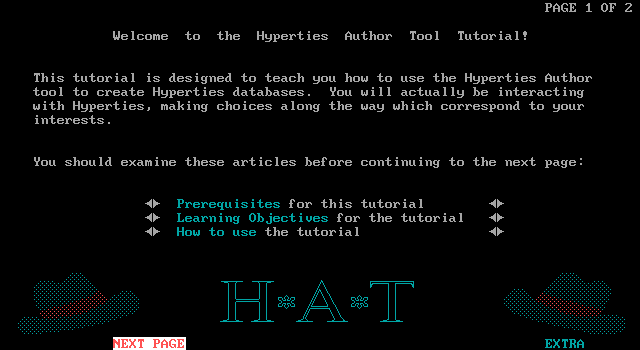
\includegraphics[width=0.7\textwidth]{images/hyperties}
\end{figure}

\end{frame}

\begin{frame}
\frametitle{HyperTIES}
\framesubtitle{Funktionen}
	\begin{itemize}
		\item Userinterface / Bedienmöglichkeiten
		\begin{itemize}
			\item Mausklick
			\item Touch Support 
			\item Pfeiltasten
		\end{itemize}
		\item Links / Strukturen
		\begin{itemize}
			\item In Artikel mit Titel und Kurzbeschreibung gegliedert
			\item Titel dient als Linktext
			\item Kurzbeschreibung dient als Preview
		\end{itemize}
	\end{itemize}
\end{frame}